\section{Software Requirement Analysis}

Software requirement analysis is a process of gathering and interpreting facts, diagnosing problems and the information to recommend improvements on the system. It is a problem solving activity that requires intensive communication between the system users and system developers. System analysis or study is an important phase of any system development process. The system is studied to the minutest detail and analyzed. The system analyst plays the role of the interrogator and dwells deep into the working of the present system. The system is viewed as a whole and the input to the system are identified. The outputs from the organizations are traced to the various processes. System analysis is concerned with becoming aware of the problem, identifying the relevant and decisional variables, analyzing and synthesizing the various factors and determining an optimal or at least a satisfactory solution or program of action.\\

\noindent A detailed study of the process must be made by various techniques like interviews, questionnaires etc. The data collected by these sources must be scrutinized to arrive to a conclusion. The conclusion is an understanding of how the system functions. This system is called the existing system. Now the existing system is subjected to close study and problem areas are identified. The designer now functions as a problem solver and tries to sort out the difficulties that the enterprise faces. The solutions are given as proposals. The proposal is then weighed with the existing system analytically and the best one is selected. The proposal is presented to the user for an endorsement by the user. The proposal is reviewed on user request and suitable changes are made. This is loop that ends as soon as the user is satisfied with proposal.\\

\noindent Preliminary study is the process of gathering and interpreting facts, using the information for further studies on the system. Preliminary study is problem solving activity that requires intensive communication between the system users and system developers. It does various feasibility studies. In these studies a rough figure of the system activities can be obtained, from which the decision about the strategies to be followed for effective system study and analysis can be taken.
\section{Software Requirement Specification}
\subsection{Functional Requirements}
\subsubsection{Students}
\begin{enumerate}
\item Login/Logout
\item Join and Create Groups
\item Private Chat with Authenticated Users
\item Send/Receive Files/Photos
\item Join Departmental Groups
\item Update Status such as online/offline/away
\item Ask queries to the chatbot
\end{enumerate}
\subsubsection{Teachers}
\begin{enumerate}
\item Login/Logout
\item Create Groups according to classes
\item Join and create new users
\item Private Chat with authenticated Users
\item Send/Receive Files
\item Update Details
\item Ask queries to the chatbot
\end{enumerate}
\subsection{Non-Functional Requirements}
\subsubsection{Databases}
A database management system that is available free of cost in the public domain should be used.
\subsubsection{Platform}
It should be software platform independent.
\subsubsection{Web Browser}
We should be able to software the product from any browser.


\section{SDLC model to be used}
There are five phases in this model and the first phase is the planning stage.  The planning
stage determines the objectives of the project and whether the project should be given the
green  light  to  proceed.   This  is  where  the  proposal  submission  comes  into  picture.\\
\noindent After
obtaining the approval, the next phase is analysis.  Gathering and analysing the system and
user requirements is essential for entry to the design step.
With the user requirements gathering completed, there is a need to prepare the resources
for the project.  Be it software or hardware components, careful consideration and selection
is to be taken care at this stage.  The decision on the appropriate resources to be used is
further elaborated under the subsections below.  The next step is to design the system and
database structure.\\ 
\noindent Results from the analysis and preparation that were concluded from the previous stage are
put into action.  With the user requirements in mind, the flow of the system is planned and
the user interface is designed to suit their easy navigation needs.  In addition, the number of
tables, attributes, primary and unique keys of the database is listed.
After  completing  the  design,  actual  coding  begins.   Database  is  created  and  codes  are
written.  Some of the codes required amendments and improvement to it so these are being
developed  at  this  fourth  stage  of  the  waterfall  model.   With  the  development  completed,
testing will begin.\\ 
\noindent The codes and database are tested to ensure the results obtained are as
intended.  More time is spent on both development and testing stages because it is inevitable
to have errors and issues and buffer time is allocated for troubleshooting.
This system will use spiral model.

\subsection{Spiral Model} 
\begin{figure}[ht]
\centering
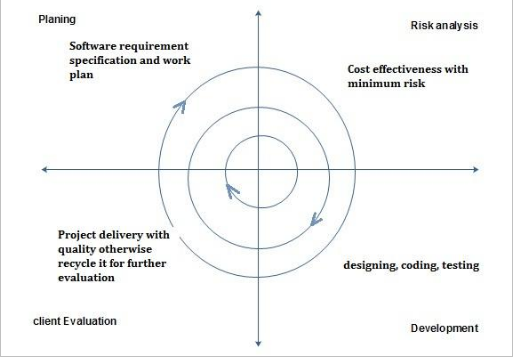
\includegraphics[scale=0.38]{input/images/sm.png}
\caption{Spiral Model}
\label{fig:Anatomy}
\end{figure}
The spiral model combines the idea of iterative development with the systematic, controlled aspects of the waterfall model. This Spiral model is a combination of iterative development process model and sequential linear development model i.e. the waterfall model with a very high emphasis on risk analysis. It allows incremental releases of the product or incremental refinement through each iteration around the spiral. It is in sync with the natural development process of any product, i.e. learning with maturity which involves minimum risk for the customer as well as the development firms.